%*****************************************
\chapter{Einf\"{u}hrung}\label{ch:introduction}
%*****************************************
Im Folgenden wird der Inhalt dieses Advanced Design Projects vorgestellt. Beginnend mit der Motivation, warum dieses Projekt ein interessantes Thema und eine nicht unwichtige Problematik darstellt und im Weiteren eine konkrete Darlegung der Aufgabenstellung der Arbeit. Im letzten Punkt werden die Methodiken der einzelnen Herangehensweisen an die verschiedenen Aufgaben und Themengebiete erl\"{a}utert. 

\section{Motivation}
Im Bereich der Fahrzeugentwicklung spielen seit Jahren Leistung und Energieverbrauch die gr\"{o}{\ss}te Rolle als Fortschrittskriterium. Durch steigende Belastung der Umwelt und der Gesundheit von Mensch und Tier, sind Umweltschutzfaktoren bei der Entwicklung von Kraftfahrzeugen immer weiter in den Vordergrund ger\"{u}ckt. Immer mehr gesetzliche Richtlinien schr\"{a}nken die Automobilhersteller in ihren Freiheiten ein und zwingen die Entwicklung in eine umweltfreundlichere Richtung. Anfangs zielte man nur auf Verbrennungsprodukte ab, die bei der Verwendung von Otto- und Dieselmotoren entstehen. Sp\"{a}ter kamen Altschrottentsorgung und Reifenabrieb hinzu. 
\\\\
Neben all diesen Faktoren ist auch die Bremse ein Bauteil im Kraftfahrzeug, welches durch Benutzung Emissionen abgibt. Da auch in diesem Teilgebiet gesetzliche Richtlinien zu erwarten sind, konzentriert sich die Forschung aktuell auf die Entstehung solcher Emissionen bei Kraftfahrzeugbremsen. Da Emissionsart und Partikelzusammensetzung der Bremsemissionen aktuell nicht gut erforscht und deshalb unbekannt sind, kann man nicht direkt Ma{\ss}nahmen gegen die Belastung durch Bremsemissionen ergreifen. Um Aufschluss \"{u}ber die Art der entstehenden Partikel zu bekommen, werden Partikelmesssysteme eingesetzt. An diesem Punkt steigt diese Arbeit ein um das zeitliche Messverhalten solcher Systeme zu \"{u}berpr\"{u}fen, damit diese sp\"{a}ter an der Kraftfahrzeugbremse eingesetzt werden k\"{o}nnen.
\section{Konkretisierung der Aufgabenstellung}
Am Fachgebiet Fahrzeugtechnik der TU Darmstadt wird in Zusammenarbeit mit der Industrie am Thema Partikelemissionen von Pkw-Scheibenbremsen geforscht. Zum Vergleich partikelemissionsarmer Bremsstrategien wird auf Grundlage von Messungen ein Partikelemissionsmodell erarbeitet. Im Rahmen der Systemidentifikation sind Informationen \"{u}ber die zeitliche Aufl\"{o}sung der verwendeten Partikelmessger\"{a}te notwendig.
\\\\
Ziel des Advanced Design Projects ist es, ein Konzept f\"{u}r eine Versuchseinrichtung zu entwickeln und dieses konstruktiv umzusetzen. Dabei ist es das Ziel die Generierung eines Partikeltestsignals in Form einer Sprungfunktion zu erm\"{o}glichen und so ein Versuchswerkzeug zur Identifizierung der zeitlichen Aufl\"{o}sung der Partikelmessger\"{a}te zu entwickeln.
\\\\
Im Einzelnen teilt sich das folgende ADP in f\"{u}nf Arbeitsschritte auf. Es beginnt mit der Einarbeitung in die Thematiken Bremspartikelemissionen, Partikelmesstechnik sowie Systemidentifikation mit Hilfe von Testsignalen. Nach der Einarbeitung in die f\"{u}r die Arbeit wichtigen Themen soll eine Ausarbeitung einer Anforderungsliste f\"{u}r die Versuchseinrichtung aufgestellt werden. Im dritten Schritt werden Konzepte f\"{u}r die Versuchseinrichtung erarbeitet um diese dann anschlie{\ss}end mit Blick auf die Anforderungsliste zu vergleichen. Am Ende wird das Konzept ausgew\"{a}hlt, welches am besten den Anforderungen entspricht. Der letzte Schritt ist eine detaillierte theoretische Konstruktion der Versuchseinrichtung.
\section{Methodik}
Zu Beginn muss gesagt werden, dass die Aufgaben nie in der Gruppe bearbeitet wurden, sondern in regelm\"{a}{\ss}igen Treffen der Gruppe besprochen und aufgeteilt wurden. Dabei wurden Milestones gesetzt, welche es termingerecht zu erreichen galt. Die erledigten Aufgaben wurden dann diskutiert und verfeinert. Anschlie{\ss}end wurden die neuen Aufgaben festgelegt, aufgeteilt und neue Milestones zu den Aufgaben gesetzt. Im Folgenden werden wir nicht weiter auf die Aufteilung der Aufgaben eingehen, da es für das Projekt keine Rolle spielt wer die Aufgaben erledigt hat, sondern es von gr\"{o}{\ss}erer Relevanz ist, wie die einzelnen Aufgaben angegangen und bearbeitet wurden.
\begin{enumerate}
\item \textbf{Einarbeitung in die verschiedenen Thematiken}:\\
F\"{u}r die Einarbeitung wurde haupts\"{a}chlich Literaturrecherche betrieben. Dabei wurde Literatur aus der Bibliothek der TU Darmstadt verwendet, welche von verschiedenen Professoren und wissenschaftlichen Mitarbeitern empfohlen wurde. Eine weitere Quelle waren die wissenschaftlichen Ver\"{o}ffentlichen der Arbeiten am Windkanal in Darmstadt und der Fachgebietes Fahrzeugtechnik an der TU Darmstadt. Auch das Internet und digitale Archiv der ULB Darmstadt wurden als Quellen f\"{u}r die Einarbeitung genutzt.
\item \textbf{Ausarbeitung einer Anforderungsliste}:\\
F\"{u}r die Erstellung einer Anforderungsliste wurde die gesamte geplante Versuchseinrichtung in verschiedene Teile unterteilt. Dabei gab es drei wichtige Aspekte der Einrichtung zu beachten. Welche Anforderungen werden aufgrund der verwendeten Messger\"{a}te vorgegeben, welche Anforderungen ergeben sich durch die Auswahl eines passenden Partikelsubstrates und welche Anforderungen entstehen f\"{u}r die eigentlichen Bauteile der Versuchseinrichtung. Dabei wurden einmal physikalische, wie auch chemische Anforderungen an Material und Aufbau gestellt, sowie allgemeine Anforderungen an das gesamte Versuchsergebnis.
\item \textbf{Entwicklung von Versuchseinrichtungskonzepten}:\\
F\"{u}r die Entwicklung von Konzepten f\"{u}r verschiedene Versuchseinrichtungen wurden f\"{u}r alle ben\"{o}tigten Elemente der Einrichtung morphologische K\"{a}sten erstellt. Die ben\"{o}tigten Elemente ergaben sich aus der Aufgabenstellung und der Anforderungsliste. Durch Brainstorming wurden die morphologischen K\"{a}sten mit verschiedenen Ideen zu einzelnen Bauteilen gef\"{u}llt. Aus den Einzelteilen entstanden in mehreren Durchl\"{a}ufen verschiedene Konzeptideen, welche skizziert und kurz beschrieben wurden. Dabei unterschieden sich die Konzepte in einem wichtigen Punkt, n\"{a}mlich in Systeme mit externen Pumpen als Antrieb und in Systeme ohne eigenen Pumpantrieb, welche von der Ansaugkraft der Messger\"{a}te abh\"{a}ngig waren. Die Konzepte wurden nach ihrer Entstehung mit wissenschaftlichen Mitarbeitern besprochen und verfeinert, wobei manche Konzepte in diesem Schritt bereits von der Liste gestrichen wurden.
\item \textbf{Vergleich der Konzepte}:\\
Mit der Anforderungsliste als Referenz wurden die \"{u}brig gebliebenen Konzepte verglichen. Dabei haben die Konzepte Punkte in jeder Anforderung bekommen. Je nach Wichtigkeit der Anforderung wogen hier die Punktzahlen mehr oder weniger. Am Ende wurde das Konzept ausgew\"{a}hlt welches, den Anforderungen am besten standhalten konnte.
\item \textbf{Auswahl und Konstruktion eines Konzeptes}:\\
Das ausgew\"{a}hlte Konzept wurde dann als detaillierte Skizze angefertigt. Nun wurden auch erste konkrete \"{U}berlegungen zu Ma{\ss}en und Materialien gemacht um eine endg\"{u}ltige Konstruktion zu entwerfen. Die Versuchseinrichtung wurde in Einzelteile zerlegt und es wurden konkrete Bauteile gefunden oder entwickelt um das bisher theoretische Konzept zu verwirklichen. Ma{\ss}e, Materialien, Herkunft und Preis der Teile wurden ermittelt und festgelegt, sodass ein fertiger Bauplan des Konzeptes vorlag.
\end{enumerate}
\section{Anforderungen}
Um sicherstellen zu k\"{o}nnen, dass das Projektziel bestm\"{o}glicht erreicht wird, wurde eine Anforderungsliste erstellt, mit deren Hilfe die G\"{u}te der Umsetzung des Versuchskonzepts gemessen werden kann. Diese Liste enth\"{a}lt die Anforderungen des Auftraggebers und unseren eigenen, welche sich aus den zu Grunde liegenden technischen Dokumenationen der verwendeten Messger\"{a}te und den VDI Richtlinien f\"{u}r Reinraumtechnik ergeben haben.\\
Bei den festgelegten Anforderungen war uns eine genaue Quantifizierung der Werte wichtig, wann immer es m\"{o}glich war. Bei den Anforderungen wird zwischen den folgenden Arten unterschieden:

\begin{enumerate}
	\item \textbf{Festforderung} (FF): Es muss ein bestimmter Wert aufweisbar sein und Abweichungen davon sind nicht zul\"{a}ssig.
	
	\item \textbf{Bereichsforderung} (BF): Die Anforderung muss einen Wert aufweisen und dieser darf nur innerhalb eines bestimmten Bereich liegen.
	
	\item \textbf{Mindestforderung} (MF): Bei einer Mindestforderung muss die Anforderung mindestens einen angegeben Wert aufweisen.
	
	\item \textbf{Zielforderung} (ZF): Der Wert einer Anforderung muss bei einer ZF m\"{o}glichst nah an einem Zielwert liegen, um gut bewertet werden zu k\"{o}nnen.
	
	\item \textbf{Wunsch} (W): Da es sich um einen Wunsch handelt, ist die Wichtigkeit des Merkmals vergleichsweise gering. Die Anforderung sollte dann allerdings einen bestimmten Wert aufweisen und wird bei der Bewertung positiv ber\"{u}cksichtigt. 
\end{enumerate}
F\"{u}r die Generierung eines Partikeltestsignals in Form einer Sprungfunktion lassen sich die folgenden Anforderungen festlegen, die sich in drei Kategorien unterteilen lassen:
\begin{enumerate}
	\item \textbf{Aerosolquelle}: Anforderungen an die Quelle, welche das Pr\"{u}faerosol erzeugt
	\item \textbf{Aerosol}: Anforderungen an das Pr\"{u}faerosol, welches dem zu testenden Messger\"{a}t zugef\"{u}hrt wird
	\item \textbf{Schaltvorrichtung}: Anforderungen an die Schaltvorrichtung, welche den Partikelsprung erm\"{o}glicht 
	\item \textbf{Aerosolleitungen}: Anforderungen an die Schnittstelle, welche die Aerosolquelle mit dem Messger\"{a}t verbindet
	\item \textbf{Versuchsaufbau}: Anforderungen an den gesamten Versuchsaufbau inklusive der verwendeten Ger\"{a}te
\end{enumerate}
\begin{longtable}{| l | l | l | l | l | l |}
	\caption{Anforderungen mit anschlie{\ss}enden Erl\"{a}uterungen}\label{anforderungsliste}\\
	\hline
	
	\textbf{Anforderung} & \textbf{Nr.} & \textbf{Art} & \textbf{Wert} & \textbf{Einheit} & \textbf{Quelle}\\

	\hline

	Druck am  & 1 & BF & Eingang - Ausgang & $kPa$ & Datenbl\"{a}tter\\
	Messger\"{a}teeinlass& & & $70 - 103$ (FMPS) & &\\
	& & & $40 - 103$ (APS) & &\\
	& & & $<0.746$ (OPS) & &\\
	& & & $75-105$ (UCPC) & &\\
	
	\hline
	
	Einstellzeit der & 2 & ZF & 0 & $s$ &selbstgew"{a}hlte\\
	Partikelanzahlkonzentration & & & & &Last\\
	der Aerosolquelle & & & & &\\
	
	\hline
	Tr\"{a}gergas& 3 & FF & & & Datenbl\"{a}tter\\
	- gefilterte Luft & & & & &\\
	
	\hline
	
	Volumenstrom & 4 & FF & 10 (FMPS) & $l/min$ & Datenbl\"{a}tter\\
	(Tr\"{a}gergas) & & & $5 \pm 0.2$ (APS)& &\\
	& & & $1 \pm 0.05$ (OPS)& &\\
	& & & $1.5 \pm 0.05$ (UCPC)& &\\
	
	\hline
	
	Tr\"{a}gergastemperatur & 5 & BF & $283.15-325.15$(FMPS) & $K$ & Datenbl\"{a}tter\\
	& & & $283.15-313.15$(APS) & &\\
	& & & $273.15-318.15$(OPS) & &\\
	& & & $283.15-308.15$(UCPC) & &\\
	
	\hline
	
	Partikelanzahlkonzentration & 6 & BF & $100-10^{7}$ (FMPS)& $n/cm^{3}$ & Datenbl\"{a}tter\\
	& & & $0,001-1000$ (APS) & &\\
	& & & $0-3000$ (OPS) & &\\
	& & & $0-3\cdot10^{5}$ (UCPC) & &\\
	
	\hline
	
	Partikelmaterial (Messger\"{a}t) & 7 & W &  &  & Datenblatt APS\\
	- feste Schwebeteilchen & & & & &\\
	
	\hline
	
	Partikelgr\"{o}{\ss}e & 8 & BF & $5.6-560$ (FMPS) & $nm$ & Datenbl\"{a}tter\\
	& & & $500-20000$ (APS) & &\\
	& & & $300-10000$ (OPS) & &\\
	& & & $2.5-3000$ (UCPC) & &\\
	
	\hline	
		
	Schaltzeit & 9 & ZF & 0 & s & selbstgew\"{a}hlte\\
	& & & & & Last\\
	
	\hline
	
	Str\"{o}mungsbeg\"{u}nstigender & 10 & ZF & 0 & n & VDI 3491\\
	Schaltvorgang & & & & &\\
	
	\hline	
			
	Weg zwischen Umschaltvorrichtung & 11 & ZF & 0 & m & selbstgew\"{a}hlte\\ 
	und Messger\"{a}teinlass & & & & & Last\\
	
	\hline
	
	Laminarer Strom (Reynoldszahl) & 12 & MF & $< 2300$ & - & VDI 3491\\
	& & ZF & $1500$ & &\\
	
	\hline
	
	Schnittstelle zum & 13 & FF & 9.5 (FMPS) & $mm$ & Datenbl\"{a}tter\\
	Messger\"{a}t (Inlet) & & & 19 (APS) & &\\
	& & & 6.35 (OPS) & &\\
	& & & 6.4 (UCPC) & &\\
	
	\hline		
		
	Pr\"{u}fzeit & 14 & ZF & 3300 & $s$ & selbstgew\"{a}hlte\\
	& & & & & Last\\
	
	\hline
	
	Kosten & 15 & ZF & 0 & Euro & Vorgabe \\
	& & BF & $0-1000$ & &\\
	
	\hline
	
	Anzahl Messger\"{a}te& 16 & MF & $\geq2$ (FMPS, OPS) & $n$ & Vorgabe\\
	
	\hline
\end{longtable}
\subsection{Aerosolquelle}
Die Aerosolquelle liefert mit dem Aerosol den entscheidenden Faktor zum Partikelsprung. Aus den Begrenzungen der Messger\"{a}te, sowie allgemeiner Richtlinien zur Aerosolgenerierung ergeben sich folgende Anforderungen:

\begin{itemize}
\item \textbf{Einhaltung eines vorgegebenen Druckbereiches(1)}\\
Die internen Pumpen, welche den Volumenstrom der Messger\"{a}te regulieren, arbeiten nur in einem bestimmten Druckbereich korrekt(Q). Dieser Druckbereich begrenzt wiederum den Aerosoldruck, welcher am Messger\"{a}t-Einlass herrschen darf. Es ist darauf zu achten, dass die Aerosolquelle diesen Druckbereich einh\"{a}lt(Q). 
Auch das Design der Aerosolleitungen und der Schaltvorrichtung beeinflussen den Druck am Messger\"{a}t-Einlass\cite{fmps_3091}\cite{ops_3330}\cite{aps_3321}\cite{ucpc_3776}\cite{tsl_skript}.

\item \textbf{Regulationszeit des Aerosolquelle(2)}\\
Die Einstellzeit einer Leistungskenngr\"{o}{\ss}e beschreibt das dynamische Verhalten der Aerosolquelle bez\"{u}glich dieser Gr\"{o}{\ss}e bei sprungf\"{o}rmigen \"{A}nderungen eines Einstellparameters. Dabei ist vor allem die Einstellzeit der Partikelanzahlkonzentration f\"{u}r den Versuchsaufbau interessant\cite{vdi3491}.

\item \textbf{Auswahl eines Tr\"{a}gergases(3)}\\
Das Tr\"{a}gergas der Aerosole hat einen gro{\ss}en Einfluss auf das Messverhalten der Messger\"{a}te.  F\"{u}r den Versuchsaufbau kommt vor allem gereinigte Luft als Tr\"{a}gergas in Frage, da diese auch bei der Messung der Bremspartikel als Tr\"{a}gergas fungiert und die ausgew\"{a}hlten Messger\"{a}te mit Luft oder Inertgas (UCPC) arbeiten\cite{fmps_3091}\cite{ops_3330}\cite{aps_3321}\cite{ucpc_3776}.

\item \textbf{Bereitstellen eines ausreichenden Volumenstroms(4)}\\
Die Messger\"{a}te arbeiten mit einem fest vorgegebenen Volumenstrom des Tr\"{a}gergases.  Es muss gew\"{a}hrleistet sein, dass die Aerosolquelle einen entsprechenden Strom bereitstellen kann. Sollte der Volumenstrom den Anforderungen nicht entsprechen, generieren die Messger\"{a}te eine Fehlermeldung und liefern keine Messwerte mehr\cite{fmps_3091}\cite{ops_3330}\cite{aps_3321}\cite{ucpc_3776}.

\item \textbf{Einhalten von Temperaturgrenzen(5)}\\ 
Die Tr\"{a}gergastemperatur kann je nach Aerosolquelle verschiedene Werte annehmen. Da die Temperatur des Aerosols den Messprozess und die Eigenschaften des Aerosolstromes beeinflusst, geben die Messger\"{a}tehersteller feste Temperaturgrenzen vor zwischen welchen sich diese Temperatur bewegen darf\cite{fmps_3091}\cite{ops_3330}\cite{aps_3321}\cite{ucpc_3776}
\end{itemize}

\subsection{Aerosol}
Folgende Anforderung an das Aerosol ergeben sich aus den Arbeitsbereichsbegrenzungen der Messger\"{a}te und aus der statistischen Verwertbarkeit der Messwerte zur Berechnung des zeitlichen Verhaltens der Messger\"{a}te.

\begin{itemize}
\item \textbf{Einhalten der Partikelanzahlkonzentration(6)}\\
Eine zu hohe Partikelanzahlkonzentration f\"{u}hrt zu einer H\"{a}ufung von falschen Messergebnissen, zum Beispiel durch Koinzidenz bei optischen Sensoren. Messergebnisse bei einer zu niedrigen Partikelanzahlkonzentration k\"{o}nnen bei Messger\"{a}ten, welche mit elektrischen Feldern arbeiten, in dem herrschenden, systematischen Grundrauschen untergehen. Somit muss f\"{u}r verwertbare Ergebnisse die Partikelanzahlkonzentration des Aerosols mit dem benutzten Messger\"{a}t abgeglichen werden\cite{fmps_3091}\cite{ops_3330}\cite{aps_3321}\cite{ucpc_3776}.

\item \textbf{Wahl des Partikelmaterial(7)} 
Partikelmaterialien k\"{o}nnen gesundheits- oder umweltgef\"{a}hrdend sein oder aufgrund von ihren Eigenschaften f\"{u}r bestimmte Messverfahren nicht geeignet sein. Deswegen ist es wichtig das benutzte Partikelmaterial zu kennen. Da die hier benutzten Messger\"{a}te vor allem f\"{u}r die Feinstaubmessung benutzt werden, bieten sich zum Beispiel feste Materialien f\"{u}r die Aerosole an\cite{vdi3491}.

\item \textbf{Wahl der Partikelgr\"{o}{\ss}e(8)}\\ 
Zu kleine Partikel k\"{o}nnen von den Messsystemen der Partikelz\"{a}hler nicht erfasst werden, w\"{a}hrend zu gro{\ss}e Partikel durch Verstopfen der Filter die Funktion beeintr\"{a}chtigen k\"{o}nnen. Manche Hersteller geben an, dass zu gro{\ss}e Partikel zwar gez\"{a}hlt werden, aber nicht mehr in die Gr\"{o}{\ss}enverteilung miteingehen. Trotzdem sollte zur Sicherheit ein Zyklonabscheider dem System zugeschaltet werden, wenn nicht garantiert werden kann, dass nicht zu viele zu gro{\ss}e Partikel im Aerosol sind\cite{fmps_3091}\cite{ops_3330}\cite{aps_3321}\cite{ucpc_3776}.
\end{itemize}

\subsection{Schaltvorrichtung}
Die Schaltvorrichtung ist das entscheidende Bauteil beim Erzeugen der Sprungfunktion. Dabei sind ein schneller Schaltprozess, aber auch ein str\"{o}mungsg\"{u}nstiges Design f\"{u}r die G\"{u}te der Schaltvorrichtung die ausschlaggebenden Kriterien. Auch das Material kann hierbei eine Rolle spielen. Folgende Anforderungen lassen sich definieren:

\begin{itemize}
\item \textbf{Erreichen einer kurzen Schaltzeit(9)}\\
Die Zeit, die die Vorrichtung ben\"{o}tigt, um von einem Schaltzustand in den anderen zu wechseln, sollte so kurz wie m\"{o}glich sein. Diese Schaltzeit tr\"{a}gt zur Totzeit des Versuchsaufbaus bei. 
	
\item \textbf{Erreichen eines Str\"{o}mungsbeg\"{u}nstigenden Schaltvorgangs(10)}\\ 
Hochwinklige Umlenkungen und abrupte Querschnitts\"{a}nderungen k\"{o}nnen zu Partikel- und Druckverlusten f\"{u}hren. Somit k\"{o}nnen sie die G\"{u}te der Partikelfront beeinflussen und sollten deswegen vermieden werden. Au{\ss}erdem kann es bei ung\"{u}nstigem Design der Schaltvorrichtung zu Turbulenzen in der Versuchseinrichtung kommen, was die Berechenbarkeit der Totzeit des Aufbaus erheblich erschwert. Die vorhergehenden \"{U}berlegungen gelten auch f\"{u}r die Auslegung der Aerosolleitung.
\end{itemize}

\subsection{Aerosolleitungen}
Auch bei der Leitung des Aerosols ist auf eine str\"{o}mungsg\"{u}nstige Auslegung zu achten. Dies betrifft die Ausma{\ss}e, das Material, den Zustand der Innenfl\"{a}chen und die r\"{a}umliche F\"{u}hrung der einzelnen Verbindungen. Die folgenden Anforderungen k\"{o}nnen also auch als Designkriterien angesehen werden.

\begin{itemize}
\item \textbf{Str\"{o}mungsweg des Versuchaufbaus(11)}\\ 
Der Weg zwischen der Umschaltvorrichtung und dem Messger\"{a}teeinlass f\"{u}hrt bei gegebenen Volumenstr\"{o}men, abh\"{a}ngig von dem benutzten Messger\"{a}t, zu einer Verz\"{o}gerungszeit, die sich in der Totzeit des Versuchsaufbaus niederschl\"{a}gt. Da das Str\"{o}mungsverhalten in den Verbindungen nur unter Annahme von Vereinfachungen zutrifft, gilt: Umso l\"{a}nger der Weg ist, umso gr\"{o}{\ss}er ist der Rechenfehler bei der Berechnung der Totzeit. Au{\ss}erdem f\"{u}hren Druck- und Partikelverluste auf diesem Weg zu einer Verzerrung der Partikelfront\cite{vdi3491}.

\item \textbf{Erreichen eines laminaren Stroms(12)}\\ 
Da eine turbulente Str\"{o}mung zu einem analytisch kaum berechenbaren Verhalten der Str\"{o}mung f\"{u}hrt, ist der Versuchsaufbau so zu gestalten, dass sich die Str\"{o}mung m\"{o}glichst \"{u}berall laminar verh\"{a}lt). Vor allem am Messger\"{a}teeinlass, wo es zu einem Querschnitts\"{u}bergang kommen kann, sollten entsprechend gestaltete Adapter daf\"{u}r Sorge tragen\cite{vdi3491}.

\item\textbf{Flexible Schnittstelle zwischen Messger\"{a}t und Versuchsaufbau(13)}\\ 
Die Messger\"{a}te besitzen einen Aerosoleinlass in Form eines R\"{o}hrchens mit unterschiedlichen Durchmessern, welches in die Umgebung ragt. Je nach Versuchsaufbau k\"{o}nnen Adapter von N\"{o}ten sein, um eine direkte Verbindung zwischen Schaltvorrichtung und Messger\"{a}t zu gew\"{a}hrleisten. Bei der Gestaltung dieser Adapter muss ein Kompromiss zwischen Anforderung 12 und 13 eingegangen werden\cite{fmps_3091}\cite{ops_3330}\cite{aps_3321}\cite{ucpc_3776}.
\end{itemize}

\subsection{Versuchsaufbau}
\begin{itemize}
\item \textbf{Optimale Pr\"{u}fzeit(14)}\\ 
Die minimale Versuchszeit ist wichtig in der Versuchsplanung, da durch die Messaufl\"{o}sung der Messger\"{a}te von einer Sekunde, die Anzahl der Messwerte je nach Versuchsaufbau begrenzt ist. Nun kann eine Versuchsdurchf\"{u}hrung aus mehreren Abl\"{a}ufen (abwechselnd: gereinigte Luft (zb. 5 s) -- Aerosol(zb. 30s)) und die Abl\"{a}ufe wiederum aus mehreren Messungen (der Partikelanzahl) bestehen. Je nach Varianz der Partikelanzahl sind eine bestimmte Anzahl von Messungen und Messabl\"{a}ufen von N\"{o}ten, um ein valides Ergebnis f\"{u}r die Zeitkonstante zu erhalten. So sollte der Aufbau ca. 100 Abl\"{a}ufe mit je 30 Partikelanzahlmessungen (+ 5 Sekunden gereinigte Luft pro Ablauf) mit reproduzierbaren Partikelspr\"{u}ngen liefern k\"{o}nnen.

\item \textbf{Annehmbare Kosten(15)}\\
Aus wirtschaftlicher Sicht sind die Kosten ein ausschlaggebender Faktor f\"{u}r die G\"{u}te des Aufbaus. Sie setzen sich aus den Materialkosten selbstgestalteter und eventuell selbstgebauter Teile, den Kosten f\"{u}r Zukaufteile, wie Filter, Verdichter, Aerosolgeneratoren etc. und den Kosten f\"{u}r Ressourcen, wie Strom, Aerosol etc., zusammen. Die maximalen Kosten d\"{u}rfen die vorgegebenen Mittel des Fachgebietes nicht \"{u}berschreiten. 

\item \textbf{Flexibilit\"{a}t f\"{u}r verschiedene Ger\"{a}te(16)}\\
Ziel des Aufbaus ist die Evaluation der Dynamik von Messger\"{a}ten, welche f\"{u}r Messungen von Bremspartikeln am Schwungmassenpr\"{u}fstand ben\"{o}tigt werden. Von den f\"{u}nf f\"{u}r diesen Zweck ausgesuchten Messger\"{a}ten wurden vor allem der FMPS 3091 und der OPS 3330 f\"{u}r geeignet befunden. Nun sollen die, durch den hier konstruierten Versuchsaufbau, ermittelten Werte zumindest f\"{u}r diese beiden Ger\"{a}te ein valides Ergebnis darstellen. Jedes weitere Messger\"{a}t, das durch den Aufbau erfolgreich getestet werden kann, erh\"{o}ht dessen wirtschaftlichen und wissenschaftlichen Wert.
\end{itemize}

%*****************************************
\chapter{Technische Grundlagen}\label{ch:foundations}
%*****************************************
F\"{u}r die Arbeit wurden verschiedene technische Grundlagen verwendet, welche im Folgenden kurz erl\"{a}utert werden sollen. Hierf\"{u}r wird auf allgemeine Elemente der Str\"{o}mungslehre sowie auf Einwirken der Reynolds- und der Prandtlzahl auf aktive Str\"{o}mungen hingewiesen. Da die Arbeit sich um die Messung von Bremsemissionspartikeln dreht, werden auch die Eigenschaften von Partikeln und Aerosolen, die f\"{u}r die Arbeit verwendet wurden kurz erkl\"{a}rt. Letztendlich werden die mechanischen Grundlagen f\"{u}r verschiedene verwendete Bauteile erl\"{a}utert und der aktuelle Stand der Technik im Bereich Aerosolstr\"{o}mung und Messtechnik aufgegriffen.

\section{Str\"{o}mungslehre}
Da es Ziel der Arbeit ist, einen konstanten Strom von Partikeln durch ein bestimmtes Medium zu generieren, um letztendlich ein Partikeltestsignal zu bekommen, ist es wichtig grundlegende physikalische Eigenschaften von Str\"{o}mungen zu kennen. Deshalb ist es unumg\"{a}nglich sich im Vorfeld mit den Grundlagen der Str\"{o}mungslehre auseinanderzusetzen.
\\\\
Die Str\"{o}mungslehre ist die Wissenschaft vom physikalischen Verhalten von Fluiden und Gasen. Die in dieser Lehre gewonnenen Kenntnisse sind Gesetzm\"{a}{\ss}igkeiten in Str\"{o}mungsvorg\"{a}ngen und dienen der L\"{o}sung von Str\"{o}mungsproblemen. Dabei liegt der Fokus auf den Problemen bei umstr\"{o}mten oder durchstr\"{o}mten Bauteilen. Gegenstand der Str\"{o}mungslehre sind die Bewegungen von Fluiden, Gasen und ruhenden, flie{\ss}enden oder str\"{o}menden Substanzen. Die Str\"{o}mungslehre l\"{a}sst sich in verschiedene Teilgebiete unterteilen, von denen allerdings f\"{u}r diese Arbeit nur die Fluiddynamik relevant ist und die Auslegungen sich daher auf dieses Teilgebiet beschr\"{a}nken werden\cite{stream}.

\subsection{Str\"{o}mungseigenschaften}
Grob betrachtet gibt es zwei wichtige Eigenschaften von Str\"{o}mungen, die f\"{u}r diese Arbeit wichtig sind. Auf der einen Seite gibt es die laminaren Str\"{o}mungen, die man sich als ein gleichm\"{a}{\ss}iges Flie{\ss}en vorstellen kann, auf der anderen Seite als Gegensatz die turbulenten Str\"{o}mungen.
\\\\
In der Fluiddynamik ist die laminare Str\"{o}mung eine Bewegung des Fluids ohne sichtbare Turbulenzen. Dabei str\"{o}mt das Fluid in Schichten, die sich nicht miteinander vermischen. Verwirbelungen treten erst mit h\"{o}heren Str\"{o}mungsgeschwindigkeiten auf, ab diesem Zeitpunkt ist die Str\"{o}mung turbulent.
\begin{figure}[H]
        \myfloatalign
        {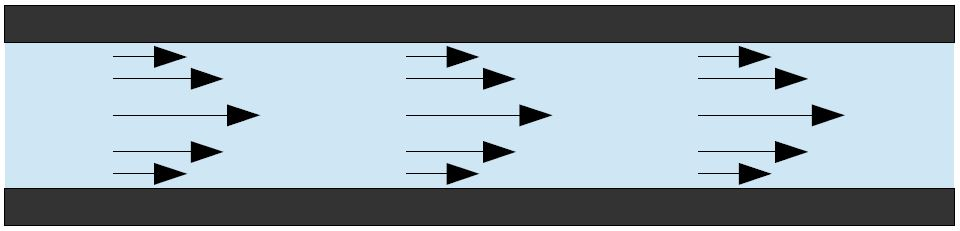
\includegraphics[width=.9\linewidth]{gfx/fundamentals/laminar.jpg}} \quad
        \caption[Laminare Str\"{o}mung]
        {Laminare Str\"{o}mung}
        \label{fig:laminar}
\end{figure}
Im Vergleich dazu ist die turbulente Str\"{o}mung die Bewegung von Fluiden, bei der Verwirbelungen auftreten. Diese Str\"{o}mungsform ist gekennzeichnet durch eine scheinbar zuf\"{a}llig variierende Komponente. Turbulenzen f\"{u}hren zu einer verst\"{a}rkten Durchmischung des Fluids mit umgebenden Gasen. Dabei hat die turbulente Str\"{o}mung eine ungeordnete und schwer vorhersagbare Struktur
\begin{figure}[H]
        \myfloatalign
        {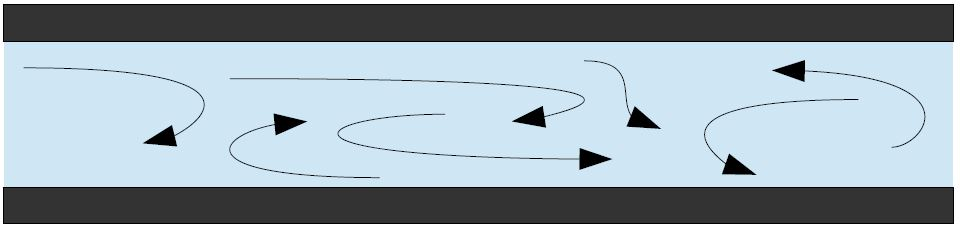
\includegraphics[width=.9\linewidth]{gfx/fundamentals/turbulent.jpg}} \quad
        \caption[Turbulente Str\"{o}mung]
        {Turbulente Str\"{o}mung}
        \label{fig:turbulent}
\end{figure}
F\"{u}r diese Arbeit wurden verschiedene Ideen mit verschiedenen Anforderungen an die Str\"{o}mung entwickelt. Gemeinsam haben alle Konzepte, dass ein laminarer Strom des Fluids am Eingang des Messger\"{a}tes verlangt war. Bei einigen kam noch hinzu, dass das Fluid vor dem Einstr\"{o}men in das Messger\"{a}t mit Luft vermischt werden sollte. Dort ist eine gezielte turbulente Str\"{o}mung gewollt, um eine Vermischung zu generieren, die im sp\"{a}teren Aufbau allerdings wieder eine laminare Form annehmen sollte\cite{stream}.
\subsection{Reynoldszahl}
Die Reynoldszahl ist eine dimensionslose Kennzahl. Sie wird in der Str\"{o}mungslehre als Beurteilungskriterium f\"{u}r laminare Str\"{o}mungen verwendet und ist deshalb relevant f\"{u}r diese Arbeit. Die Reynoldszahl ist definiert durch:
\begin{align*}
{Re} = \frac{\rho vd}{\eta} = \frac{vd}{\nu}
\end{align*}
Dabei ist \(\rho\) die Dichte des Fluids, \(v\) die Str\"{o}mungsgeschwindigkeit des Fluids gegen\"{u}ber dem durchstr\"{o}mten K\"{o}rper und \(d\) die L\"{a}nge des K\"{o}rpers. Die kinematische Viskosit\"{a}t \(\nu\) des Fluids unterscheidet sich von der dynamischen Viskosit\"{a}t \(\eta = \nu \rho\) durch den Faktor \(\rho\). \"{U}berschreitet die Reynoldszahl einen kritischen Wert \({Re}_{krit}\), wird eine bis dahin laminare Str\"{o}mung anf\"{a}llig gegen kleinste St\"{o}rungen und aus der laminaren Str\"{o}mung wird eine turbulente Str\"{o}mung. In Bezug auf die Arbeit war es also wichtig eine Reynoldszahl zu erreichen, die dem verlangten Str\"{o}mungsbild gen\"{u}gt\cite{reynolds}.
\section{Partikeleigenschaften}
Die in dieser Arbeit verwendeten Partikel sind mineralische und organische Feststoffe, die nicht in L\"{o}sung gehen und wegen ihrer geringen Gr\"{o}{\ss}e und damit geringen Gewichts in der Schwebe gehalten oder durch geringe Bewegungen des Mediums verteilt werden. Im speziellen sind das hier Aerosolpartikel, St\"{a}ube und auch Nebel- und Rauchpartikel.\\
Die Eigenschaft von Partikeln, \"{u}ber l\"{a}ngere Zeit in Gasen transportiert werden zu k\"{o}nnen, liegt darin, dass sie sich mit abnehmendem Durchmesser immer mehr wie Gas Molek\"{u}le verhalten.\\
Partikel entstehen durch verschiedene Vorg\"{a}nge, welche ausschlaggebend f\"{u}r die Gr\"{o}{\ss}e der Partikel sind. Die kleinsten Partikel entstehen durch Verbrennungen und sind selten gr\"{o}{\ss}er als \(1 nm\). Mineralstaubpartikel hingegen gehen auf Abrieb mineralischer Stoffe zur\"{u}ck und sind meist von gr\"{o}{\ss}erer Form im \(\mu m\) Bereich.\\
Partikel k\"{o}nnen vom Menschen eingeatmet werden, dabei bleiben bis zu 10\% der Partikel im Atemtrakt h\"{a}ngen und f\"{u}hren so zu einer großen Belastung in Lungen und Bronchien. Da es abh\"{a}ngig von der Partikelgr\"{o}{\ss}e ist, ob und wie sch\"{a}dlich die Partikel sind, ist es wichtig durch Messungen zu erfahren welche Eigenschaften und Aufbau die Partikel haben, die durch den Bremsvorgang entstehen.
\newpage

\subsection{Bremsemissionspartikel}
Die Emissionspartikel von Bremsen  sind Bestandteil des Bremsstaubes, welcher beim Bremsvorgang entsteht. Sie stellen ein Gemisch aus Bremsbelagabrieb und Abrieb der Bremsscheiben dar, wobei der gr\"{o}{\ss}ere Anteil auf die Bremsbel\"{a}ge f\"{a}llt, da diese wesentlich weicher sind. Kritisch beim Bremsstaub sind die Partikel von Eisen, Kupfer und Mangan, die beim scharfen Bremsen freigesetzt werden. Die toxische Wirkung der einzelnen Partikel k\"{o}nnen Entz\"{u}ndungen in den Lungenzellen verursachen.\\
Da es auf das Bremsverhalten ankommt, welche Partikel in welchen Massen entstehen, ist es wichtig die entstehenden Partikel bei verschiedenen Bremsvorg\"{a}ngen zu messen und zu analysieren. Nur dann kann man gezielt Partikel bestimmter Art und Sorte reduzieren oder abfangen. So ist zum Beispiel das krebserregende Asbest auch aus der Entwicklung von Bremsscheiben herausgenommen worden.

\subsection{Partikelmessverfahren}
Unter dem Begriff Partikelmessung wird eine Gruppe von Messverfahren zur Qualifizierung und Quantifizierung von Partikeln unterschiedlicher Natur zusammengefasst. Dabei wird meistens das Prinzip des Streulichtpartikelmessung angewendet. Bei der Streulichtpartikelmessung wird eine definierte Menge einer Probe durch einen Laserstrahl gef\"{u}hrt. Das Licht des Laserstrahls bricht sich an den Partikeln oder wird von ihnen absorbiert. Photodioden k\"{o}nnen diese Effekte messtechnisch erfassen und in ein elektrisches Signal umwandeln. Dieses Signal wird von einem Computer mit einem zuvor aufgenommenen Signal verglichen, bei dem Latexkugeln definierter Gr\"{o}{\ss}e vermessen worden sind, um Referenzwerte zu schaffen. Mit diesen Daten ist man in der Lage aufgrund von statistischen Methoden die Anzahl der Partikel in einem Kubikmeter Luft oder Gas zu ermitteln. Dieses Verfahren funktioniert allerdings nur f\"{u}r Partikel mit einer Gr\"{o}{\ss}e von unter \(25 \mu m\).

\subsection{Aerosole}
Ein Aerosol ist ein heterogenes Gemisch aus festen oder fl\"{u}ssigen Partikeln in einem Gas. Ein Aerosol ist ein dynamisches System und unterliegt st\"{a}ndigen \"{A}nderungen durch Kondensation von D\"{a}mpfen an bereits vorhandenen Partikeln, Verdampfen fl\"{u}ssiger Bestandteile der Partikel oder Abscheidung von Teilchen an umgebenden Gegenst\"{a}nden.\\
Aerosole k\"{o}nnen durch mechanische Zerkleinerung von Material oder durch Kondensation von Material entstehen. Mechanische Prozesse umfassen Zerreiben, Zerstoßen oder andere Zerkleinerungsprozesse von Feststoffen. Kondensation hingegen ist ein Prozess, in dem sich festes oder fl\"{u}ssiges Material aus \"{u}bers\"{a}ttigten Gasen bildet.
\\\\
Der Durchmesser von Aerosolpartikeln liegt in der Gr\"{o}{\ss}enordnung zwischen \(0,1 nm\) und \(10 \mu m\) und sie haben unterschiedliche Zusammensetzungen. Kleinste Partikel sind einzelne Molek\"{u}le, die bei Verbrennungen entstehen.
\\\\
Angewendet werden Aerosole gro{\ss}fl\"{a}chig in der Industrie als Spraybasis, zum Auftragen von Lacken, medizinische Sprays und als Industriek\"{u}hlmittel. Um f\"{u}r die Zwecke dieser Arbeit einen Partikelsprung zu erzeugen hat sich ein Aerosol als Partikeltr\"{a}ger angeboten, da die Partikel in Aerosolen gleich verteilt sind und zu laminaren Str\"{o}mungen neigen.
\section{Mechanische Grundlagen}
In den vorgestellten Konzepten werden verschiedene mechanische Bauteile verwendet. Dabei werden einfache Teile wie Rohre, Klemmen und Schl\"{a}uche als trivial angenommen und es wird nicht weiter auf die Eigenschaften dieser Teile eingegangen. Kompliziertere Bauteile sollen hier allerdings kurz erl\"{a}utert werden, um das Verst\"{a}ndnis f\"{u}r deren Funktion zu vereinfachen und die Anwendung zu verstehen.
\\\\
Da der aufgebaute Aerosolstrom durch ein System von mehreren Rohren und Schl\"{a}uchen geleitet werden muss und gegebenenfalls auch umgeleitet werden muss, wird ein Ventil ben\"{o}tigt. Ein weiteres Bauteil sind Luftfilter, um die zum Mischen verwendete Umgebungsluft zu reinigen. Letztendlich werden noch Str\"{o}mungsmaschinen f\"{u}r einige Konzepte ben\"{o}tigt, um dem Strom eine konstante Geschwindigkeit zu geben.

\subsection{Ventile}
Ein Ventil ist ein Bauteil zur Absperrung oder Regelung des Durchflusses von Fluiden. Innerhalb des Bauteils wird ein Verschlussteil nahezu parallel zur Str\"{o}mungsrichtung des Fluids bewegt. Die Str\"{o}mung kann reduziert oder unterbrochen, indem das gesamte Verschlussteil an eine passend geformte \"{O}ffnung gepresst wird. Ventile haben die Eigenschaft \"{u}ber den gesamten Stellbereich ein gleichm\"{a}{\ss}iges Str\"{o}mungsbild zu besitzen, weshalb sie sich gut f\"{u}r Regelaufgaben eignen.
\\\\
Ventile lassen sich in vier Kategorien einteilen. Durchgangsventile reduzieren Str\"{o}mungen und der Eintritt liegt in der selben Richtung wie der Austritt. Eckventile leiten den Strom um, indem Ein- und Austritt im rechten Winkel zueinander liegen, w\"{a}hrend Schr\"{a}gventile die Str\"{o}mungsrichtung um \(45^\circ\) \"{a}ndern. Die f\"{u}r diese Arbeit wichtigen Ventile sind Drei-Wege-Ventile, die f\"{u}r das kontrollierte Mischen von Fluidstr\"{o}men verwendet werden. Bei allen Kategorien kann man noch Unterschiede in den Bet\"{a}tigungsarten machen, um jedoch ein Signal f\"{u}r den Messbereich zu haben, werden hier elektronische Bet\"{a}tigungen bevorzugt\cite{ventil}.
\begin{figure}[H]
        \myfloatalign
        {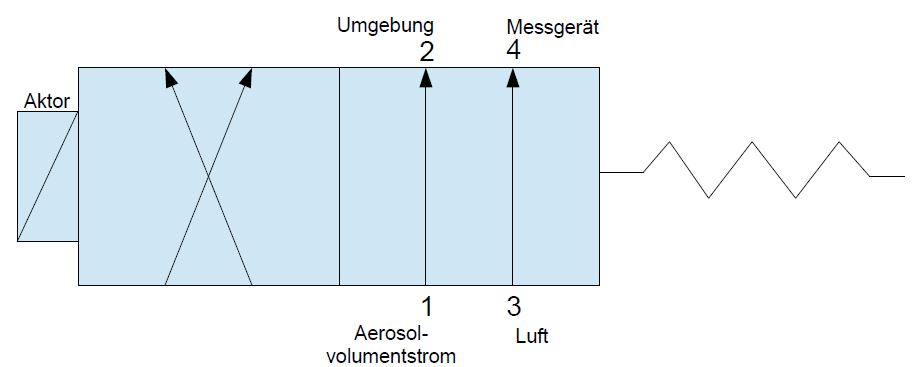
\includegraphics[width=.9\linewidth]{gfx/concepts/ventil_feder.jpg}} \quad
        \caption[Schaltm\"{o}glichkeiten von 4/2-Wegeventilen]
        {Schaltm\"{o}glichkeiten von 4/2-Wegeventilen}
        \label{fig:ventil}
\end{figure}

\subsection{Luftfiltersysteme}
Als Luftfilter werden alle Abscheider bezeichnet, die Aerosole oder andere unerw\"{u}nschte Schwebstoffe aus der Luft herausfiltern. Es gibt viele verschiedene Bauarten von Luftfiltersystemen, doch es werden nur Trockenfilter, Zyklonabscheider und elektrostatische Luftfilter verwendet, weshalb die fl\"{u}ssigkeitsbasierten Filter hier nicht wieder erw\"{a}hnt werden. \\
Trockenfilter bestehen aus ringf\"{o}rmig oder rechteckig angeordneten Gebilde, die zickzackf\"{o}rmiges Gewebe als Filterelement haben. Die Faltung vergr\"{o}{\ss}ert die Filterfl\"{a}che und verringert den Str\"{o}mungswiderstand. Die kontaminierte und ungefilterte Luft wird ausserhalb des Zylinders angesaugt und die gefilterte saubere Luft wird innerhalb der Lamellen weitergeleitet. Die Partikel und Schwebeteilchen bleiben in den Gewebefalten h\"{a}ngen.\\
Elektrofilter finden haupts\"{a}chlich Anwendung bei der Abscheidung von Aerosolen. Im Filter werden die Staub- oder Aerosolpartikel elektrostatisch aufgeladen und an den Elektrodenfl\"{a}chen abgeschieden. In getakteten Abfolgen werden die aufgefangenen Verschmutzungen maschinell entfernt und in einem Trichter gesammelt. Der Vorteil dieser Filter im Vergleich zu den Trockenfiltern ist, dass es keine Filtereins\"{a}tze gibt, die ausgetauscht werden m\"{u}ssen, allerdings sind die elektrostatischen Filter wesentlich teurer als die Einwegfilter mit Gewebeeinsatz.\\
Zyklonabscheider werden dazu genutzt, um Partikel einer bestimmten Gr\"{o}{\ss}e aus dem Strom herauszufiltern. Diese finden ihre Anwendung, um nur Partikelgr\"{o}{\ss}en durchzulassen, die f\"{u}r die verwendeten Messger\"{a}te erkennbar sind. Sie sind allerdings zu ineffizient, um die Luft von allen Partikeln zu reinigen, weshalb sie nur zur Aufbereitung des Partikelstroms in Frage kommen\cite{filter}.

\subsection{Str\"{o}mungsmaschinen}
Da es eines der Ziele ist, einen konstanen Partikelstrom durch den Versuchsaufbau zu leiten, wird eine Str\"{o}mungsmaschine ben\"{o}tigt, um den Strom in Bewegung zu bringen. Daf\"{u}r gibt es verschiedene M\"{o}glichkeiten. F\"{u}r fl\"{u}ssige und feste Stoffe werden Pumpen verwendet, die bei der Str\"{o}mungserzeugung eine Druckerh\"{o}hung mit sich bringen. Auch wenn in vielen Messger\"{a}ten laut Datenblatt die Luft mit Pumpen angezogen wird, werden dort keine Pumpen verwendet, sondern sogenannte Verdichter. Verdichter saugen durch ein Vakuum Gase an und erzeugen so Str\"{o}mungen. Allerdings ist auch hier eine Druckerh\"{o}hung unvermeidbar. Um keine hohen Dr\"{u}cke in den Leitungen zu haben, werden Gebl\"{a}se, oder Ventilatoren verwendet. Die Ventilatoren erzeugen durch ein angetriebenes Laufrad einen Luftstrom und erzeugen so eine Str\"{o}mung in die man nun das Gas einflie{\ss}en lassen kann\cite{maschine}.
\section{Signaltechnik}
Da es in dieser Arbeit darum geht einen Signalsprung zu erzeugen, wird noch einmal die grundlegende Theorie zu Sprungfunktionen und Signalzeiten erl\"{a}utert. Nach der Definition ist ein Signal ein Zeitpunkt zu dem ein wichtiges Ereignis eintritt. In diesem Fall ist das Ereignis ein Partikelsprung. Als Messstelle wird der optische Z\"{a}hler im Messger\"{a}t verwendet, an dem die eigentliche Messung der Partikel stattfindet. Zu Beginn des Systems enth\"{a}lt das Gas, welches den Z\"{a}hler passiert in der Theorie keine Partikel. Der Partikelanteil liegt also bei \(0\) Partikel \(/\) \(1m^3\) Luft. Ist der Partikelstrom komplett aufgebaut und wird in das Messger\"{a}t geleitet, beschreibt der Partikelanteil im Strom einen Sprung auf einen angestrebten Wert.
\\
Bei diesem Vorgang sind allerdings einige Zeiten zu beachten, welche das System und die entstehende Sprungfunktion beeinflussen. Zun\"{a}chst einmal hat das Messger\"{a}t eine Totzeit, welche die Zeit beschreibt, die ein Partikel vom Eingang des Messger\"{a}ts bis zum Zeitpunkt seiner Messung ben\"{o}tigt. Also bis zu dem Zeitpunkt in dem das Auftreten des Partikels in der Sprungfunktion sichtbar wird. Eine weitere Zeitspanne, die ber\"{u}cksichtigt werden muss, ist die Schaltzeit eines Ventils. Nachdem der Strom voll aufgebaut ist, muss der Luftstrom, der in das Messger\"{a}t einstr\"{o}mt umgeschaltet werden auf den aufgebauten Partikelstrom. Dieses Umschalten kostet auch Zeit, je nachdem welcher Schaltmechanismus verwendet wird. Zusammen genommen ergeben die beiden Zeiten die Totzeit des gesamten Systems. Beschrieben wird die Zeitspanne vom Umschalten des Schaltmechanismus bis zum ersten Anstieg der gemessenen Sprungfunktion.
\section{Stand der Technik}
W\"{a}hrend der Einarbeitungszeit sind wir durch Literaturrecherche auf einige Dissertationen, Abschlussarbeiten und Richtlinien aufmerksam geworden, welche vergleichbare Versuchsaufbauten beinhalten, weche haupts\"{a}chlich zur Kalibrierung von Partikelmessger\"{a}ten dienen.
\\
\\
Die Masterarbeit \ref{xyz} hatte das Ziel das Ansprechverhalten einer Constant Volume Sampling (CVS) Anlage zu optimieren. Der daf\"{u}r verwendete Versuchsaufbau ist in Abbildung \ref{aufbau_graz} abgebildet. Das hierf\"{u}r verwendete Aerosol wurde aus den Abgasen eines Versuchsfahzeugs entnommen und zusammen mit Verd\"{u}nnungsluft in einen CVS Tunnel geleitet, in welchem sich ein Partikelmesssystem befindet. Die Partikeltestsignale wurden hierbei mit Hilfe eines Umschalters erzeugt, bei dem zwischen einem Aerosolstrom und Luftstrom geschaltet werden kann (Abbildung \ref{umschalter_graz}). Diese M\"{o}glichkeit der Generierung eines Partikeltestsignals wurde in die Erarbeitung von unseren Konzepten miteinbezogen. Zudem k\"{o}nnte der CVS Tunnel f\"{u}r nachfolgende Arbeiten, welche sich ausschlie{\ss}lich mit den Str\"{o}mungen der Aerosole besch\"{a}ftigen w\"{u}rde, von Interesse sein.
\\
\begin{figure}
	\centering
	\caption{Pr\"{u}fstand der TU Graz}
	\label{aufbau_graz}
\end{figure}

\begin{figure}
	\centering
	\caption{Umschaltvorgang des Pr\"{u}fstands der TU Graz}
	\label{umschalter_graz}
\end{figure}
Auf direkte Nachfrage hin beim Hersteller der Partikelmessger\"{a}te, wie die angegebenen Werte in den technischen Dokumentationen verifiziert wurden, wiesen diese lediglich darauf hin, dass die Partikelmessger\"{a}te mit Hilfe von Aerosolgeneratoren kalibriert werden. Dies entspricht der Standardvorgehensweise zur Kalibrierung solcher Messger\"{a}te, wie sie in den VDI Richtlinien zu finden sind. Aus diesen liesen sich Kenngr\"{o}{\ss}en und Richtlinien an die zu verwendeten Aerosolgeneratoren ableiten, welche in der Reinraumtechnik Verwendung finden.
\\
\\
Uns sind letzendlich keine Versuchsaufbauten bekannt, welche ausschlie{\ss}lich zur Identifizierung der Zeitkonstante eines Partikelmessger\"{a}ts dienen. Zudem lies sich die Zeitkonstante aus keinem der uns vorliegenden Handb\"{u}cher entnehmen die darauf hindeuten w\"{u}rden, dass es ein existierendes Verfahren gibt diese zu messen. 

%************************************************
\chapter{Vergleich von Pr\"{u}f-Aerosole}\label{ch:aerosol}
%************************************************
Ein Pr\"{u}faerosol ist ein Aerosol f\"{u}r das je nach Verwendungszweck relevante Eigenschaften bekannt sind. Es kann auf verschiedene Art und Weisen hergestellt werden und dient unter anderem zur Kalibrierung von Partikelmessger\"{a}ten und f\"{u}r Filtertests.\\
Die Herstellung eines Pr\"{u}faerosols erfolgt in mehreren Schritten. Es beginnt mit der konstanten Zuf\"{u}hrung des Partikelmaterials, gefolgt von der eigentlichen Partikelproduktion. War das Partikelmaterial hochkonzentriert, findet am Ende meist noch eine Verd\"{u}nnung statt. Herstellungsmethoden sind Zerst\"{a}ubung von Feststoffen, Vernebeln von Fl\"{u}ssigkeiten, Kondensationsverfahren oder Verbrennungsprozesse.\\
Da f\"{u}r einige Konzepte Partikelgeneratoren zum Einsatz kommen, ist es wichtig die g\"{a}ngstigen Pr\"{u}faerosole kurz zu analysieren um das passendste Aerosol auszuw\"{a}hlen.

\section{Di-Ethyl-Hexyl-Sebacat (DEHS)}
Di-Ethyl-Hexyl-Sebacat (DEHS) ist ein Gemisch aus drei isomeren chemischen Verbindungen aus der Gruppe der Carbons\"{a}ureester. Erzeugt wird die Fl\"{u}ssigkeit durch einen S\"{a}urekatalysator oder durch hohen Druck. DEHS ist brennbar, aber schwer entz\"{u}ndbar, farb- und geruchlos und praktisch unl\"{o}slich in Wasser. Verwendung findet es als Weichmacher, Schmierstoff und zur Erzeugung stabiler Pr\"{u}faerosole. DEHS ist aktuell das g\"{a}ngstige Partikelmaterial in Industrie und Forschung, da es gesundheitlich unbedenklich ist und in einem gro{\ss}en Temperaturbereich stabil ist. Je nach Generator ist eine gro{\ss}e Spannbreit an Partikelgr\"{o}{\ss}en m\"{o}glich.
\begin{itemize}
\item Aggregatzustand: fl\"{u}ssig
\item Dichte: \(0,91 g/cm^3\)
\item Schmelzpunkt: \(-55^\circ\text{C}\)
\item Siedepunkt: \(256^\circ\text{C}\)
\item Partikelgr\"{o}{\ss}e: Abh\"{a}ngig vom Generator
\end{itemize}
\section{Di-N-Octylphtalat (DOP)}
Di-N-Octylphtalat (DOP) ist eine organische Verbindung aus der Gruppe Phtalate. Es ist eine farblose, geruchlose und \"{o}lige Fl\"{u}ssigkeit. DOP wird durch die Reaktion von Phtalats\"{a}ureanhydrid und Octanol in Gegenwart eines Katalysators gewonnen. Wie DEHS ist DOP in Wasser kaum l\"{o}slich. Auch in der Anwendung deckt DOP dasselbe Gebiet ab, dar\"{u}ber hinaus findet es allerdings noch Anwendung im medizinischen Bereich und in der Sprengstoffindustrie. DOP z\"{a}hlt als stark krebserregend, weshalb es nicht mehr als Weichmacher f\"{u}r Verbrauchsgegenst\"{a}nde verwendet werden darf. Auch hier wird eine gro{\ss}e Spannbreite an Partikelgr\"{o}{\ss}en abgedeckt, je nachdem welcher Partikelgenerator verwendet wird.
\begin{itemize}
\item Aggregatzustand: fl\"{u}ssig
\item Dichte: \(0,98 g/cm^3\)
\item Schmelzpunkt: \(-49^\circ\text{C}\)
\item Siedepunkt: \(385^\circ\text{C}\)
\item Partikelgr\"{o}{\ss}e: Abh\"{a}ngig vom Generator
\end{itemize}
\section{Emery 3004 (PAO-4)}
%TODO
\section{Poly Styrene Latex Spheres (PSL)}
%TODO
\section{Auswertung der Analyse}
%TODO

\subsection{Anforderungsvergleich der Aerosole}
%TODO

%************************************************
\chapter{Konzepte f\"{u}r den Versuchsaufbau}\label{ch:concepts}
%************************************************
\section{Partikelgeneratoren}
F\"{u}r die Kalibrierung und Pr\"{u}fung von Partikelmessger\"{a}ten werden oft industrielle Partikelgeneratoren verwendet. Diese Generatoren arbeiten auf Basis von Vernebelung oder Verdampfung von Fl\"{u}ssigkeiten. Die Fl\"{u}ssigkeiten werden unter hohem Druck in einer D\"{u}se vernebelt und verspr\"{u}ht oder sie werden durch hohe Temperaturen verdampft. Dabei entsteht ein Aerosol, welches Partikel der verwendeten Fl\"{u}ssigkeit enth\"{a}lt. Um die Messger\"{a}te gezielt kalibrieren zu k\"{o}nnen, kann bei den Generatoren die gew\"{u}nschte Dichte sowie die Gr\"{o}{\ss}e der Partikel innerhalb des Aerosols reguliert werden. So hat man zu jedem Zeitpunkt Kenntnis \"{u}ber den Aufbau des Partikelstroms. Da sich in dieser Arbeit auf die Verwendung von DEHS Aerosol beschr\"{a}nkt wird, werden nur die beiden Generatoren in Erw\"{a}gung gezogen, welche DEHS unterst\"{u}tzen. Dies sind auch die beiden Ger\"{a}te, welche in der Industrie am meisten vorkommen und verwendet werden.

\subsection{Topas ATM 220}
Die Ger\"{a}tereihe ATM von Topas wird schon seit langer Zeit speziell im Bereich der Reinraum- und Filtertestanwendung verwendet. Das Kernst\"{u}ck des Generators ist ein Edelstahlatomizer, eine nach dem Injektorprinzip arbeitende Zweistoffd\"{u}se. Dieser sorgt f\"{u}r die R\"{u}ckf\"{u}hrung der bei der Verd\"{u}sung entstehenden gro{\ss}en Tropfen, welches die Partikelkonzentration nur unwesentlich beeinflusst. Die f\"{u}r die Verd\"{u}sung ben\"{o}tigte Druckluft wird durch einen HEPA-Filter gereinigt. Die D\"{u}se ist direkt in die Fl\"{u}ssigkeit getaucht, um auch sehr geringe Massestr\"{o}me reproduzierbar einstellen zu k\"{o}nnen.\\
Der Topas ATM hat eine Partikelmengenspannbreite  von \(10^5\) bis \(10^8\) Partikel pro \(cm^3\), bei einer Gr\"{o}{\ss}enverteilung von \(0,1 - 0,5 \mu m\).\cite{topas}

\subsection{Palas 2000H}
Der Palas 2000H wird nicht nur f\"{u}r die Kalibrierung von Partikelmessger\"{a}ten sondern auch zum Testen von Filtersystemen verwendet. Im Gegensatz zum ATM arbeitet der Palas mit Hilfe von Kondensation und Verdampfung. So kann durch Druck- und Temperatur\"{a}nderungen die Partikelgr\"{o}{\ss}enverteilung reguliert werden. Der gro{\ss}e Vorteil des Palas 2000H ist, dass er \"{u}ber Ethernet von einem Computer aus gesteuert werden kann und somit direkt in ein Evaluationsprogramm f\"{u}r den Versuchsaufbau eingebunden werden kann. Er ist wesentlich nutzerfreundlicher als der f\"{u}r den Fachmann entwickelte ATM, erzeugt aber wesentlich gr\"{o}{\ss}ere Partikel, die f\"{u}r den Versuchsaufbau gar nicht ben\"{o}tigt werden. Au{\ss}erdem arbeitet der Generator mit einer Temperaturregelung und erhitzt das erzeugte Aerosol auf diesem Weg, welches sich nachteilig auf das Verhalten der Str\"{o}mung auswirken kann. Die Partikelmenge kann nicht eingestellt werden und liegt bei \(10^6\) Partikeln\(/cm^3\) bei einer regulierbaren Gr\"{o}{\ss}enverteilung von \(0,2 \mu m - 100\mu m\).\cite{palas}
\section{Morphologischer Kasten f\"{u}r die Konzepte}
\section{Konzept 1.1}
Das erste Konzept basiert auf der Verwendung von industriellen Partikelgeneratoren und mechanischen Ventilen. Hierbei gibt es zwei M\"{o}glichkeiten den Strom zu erzeugen, die im Folgenden n\"{a}her erl\"{a}utert werden sollen. Der Fokus liegt bei diesen Konzepten auf dem Rohrsystem, da die eigentlichen Bauteile bereits funktionsf\"{a}hig gekauft werden und nur verbaut werden m\"{u}ssen.

\subsection{Aufbau}
Der Versuchsaufbau besteht aus einer Parallelschaltung eines Aerosolgenerators mit einem Ventilator. Der Ventilator erzeugt einen reinen Luftstrom der mit dem Aerosolstrom in das selbe Rohr geleitet wird. In diesem Rohr ist eine Mischvorrichtung installiert, welche aus Luft- und Aerosolstrom eine homogene Mischung erzeugt. Das Rohr endet am Anschluss(\textit{Anschluss 1}) eines 4/2 - Wegeventils (\textit{Abbildung x.x}). Ein Ausgang des Ventils (\textit{Anschluss 2}) f\"{u}hrt raus in die Umgebungsluft, \textit{Anschluss 4} f\"{u}hrt \"{u}ber einen Adapter direkt an den Einlass des Messger\"{a}tes. Dabei ist es wichtig, darauf zu achten, dass die Verbindung zwischen Ventil und Messger\"{a}t so kurz wie m\"{o}glich gehalten wird um die Totzeit des Systems klein zu halten. Dennoch muss es mindestens so lang sein um einen moderaten Querschnitts\"{u}bergang zu gew\"{a}hrleisten, um Druck- und Partikelverluste zu minimieren. \textit{Anschluss 3} des Ventils ist mit einem weiteren Ventilator verbunden, welcher auch einen reinen Luftstrom erzeugt. Dieser Luftstrom ist für die Nullphase des Messger\"{a}tes gedacht.

\subsection{Funktionsweise}
Der Aerosolgenerator generiert einen konstanten Partikelmassenstrom mit einstellbaren Partikeleigenschaften wie die Konzentration oder die Gr\"{o}{\ss}enverteilung der Partikel. Zusammen mit der Luft aus dem externen Ventilator kann die Partikelkonzentration zus\"{a}tzlich nochmal reguliert werden und der Aerosolstrom dem angeschlossenen Messger\"{a}t angepasst werden. Die anschlie{\ss}ende Mischvorrichtung sorgt f\"{u}r eine gleichm\"{a}{\ss}ige \"{u}ber den Rohrquerschnitt verteilte Partikelkonzentration sowie eine laminare Str\"{o}mung beim Eintritt in das Ventil. Der Vorteil davon liegt darin, dass manche Messger\"{a}te dem Volumenstrom noch vor dem Passieren der Messkammer einen Schleierstrom (\textit{Sheath-Air}) entnehmen, da dieser abgezweigte Strom bei hohem Konzentrationsgradienten in radialer Richtung zu starken Schwankungen in der Konstanz des Partikelstroms f\"{u}hren kann. Das 4/2 - Wegeventil zeichnet sich durch vier Anschl\"{u}sse und zwei Schaltstellungen aus. Dabei ist in der stabilen Position (\textit{Stellung 0}) \textit{Anschluss 1} direkt mit \textit{Anschluss 2} verbunden. Dementsprechend f\"{u}hrt \textit{Anschluss 3} zu \textit{Anschluss 4}, welcher in das Messger\"{a}t m\"{u}ndet. In der monostabilen Stellung (\textit{Stellung 1}) f\"{u}hrt der Aerosolstrom (\textit{Anschluss 1}) direkt zum Messger\"{a}t (\textit{Anschluss 4}) und der Anschluss des Ventilators (\textit{Anschluss 3}) f\"{u}hrt direkt \"{u}ber \textit{Anschluss 2} in die Umgebungsluft. Das Ventil kann dabei elektronisch oder pneumatisch geschaltet werden. Der extern angetriebene Ventilator treibt Umgebunsluft durch einen Nullfilter zu dem jeweils geschalteten Anschluss. Dabei ist wichtig, dass der Volumenstrom der reinen Luft dem ben\"{o}tigten Volumenstrom des Messger\"{a}tes entspricht. Der Nullfilter sorgt f\"{u}r einen hohen Partikelkonzentrationsunterschied des Messger\"{a}teeinlassstroms zwischen Stellung 0 und Stellung 1 des Ventils.

\subsection{Durchf\"{u}hrung}
Als erstes stellt man den externen Ventilator an \textit{Anschluss 3} auf den Volumenstrom des Messger\"{a}tes ein und schlie{\ss}t das Messger\"{a}t dann \"{u}ber den Adapter an \textit{Anschluss 4} an.\\
Die Vorlaufzeit, also die Zeit bevor das Ventil geschaltet wird, h\"{a}ngt von mehreren Faktoren ab. So hat das Messger\"{a}t eine Einlaufzeit, nach der es erste zuverl\"{a}ssige Ergebnisse liefert. Nach Ablauf dieser Nullzeit wird das Messger\"{a}t weiter mit dem durch den Ventilator angetriebenen Luftvolumenstrom durchstr\"{o}mt. Parallel dazu laufen der Aerosolgenerator und der andere Ventilator, bis sie die gew\"{u}nschten Stromeigenschaften liefern. Diese Laufzeit ist vor allem von der Einstellzeit des Aerosolgenerators abh\"{a}ngig, welche die Anpassung eines Ausgangsparameters auf eine \"{A}nderung eines Eingangsparameters beschreibt. Nachdem die Voraussetzungen eines eingelaufenen Messger\"{a}tes und eines konstanten Aerosolstroms erf\"{u}llt sind, kann das Ventil geschaltet werden und der korrigierte Verlauf der Sprungantwort mit dem Eingangssignal verglichen werden. Die Korrektur betrifft hierbei die Berechnung der systematischen Totzeit des Versuchsaufbaus, welche sich aus der Schaltzeit des Ventils und der Zeit, welche die Partikelfront braucht um den Messger\"{a}teeinlass zu erreichen, zusammensetzt.

\subsection{Variation: Konzept 1.2}
Der Aufbau des ersten Konzeptes l\"{a}sst sich stark vereinfachen, wenn Messger\"{a}te benutzt werden, welche mit geringen Volumenstr\"{o}men arbeiten. Der geringe Volumenstrom ist alleine durch den Aerosolgenerator ohne einen externen Ventilator erreichbar. Somit ist auch die Mischvorrichtung zur Homogenisierung \"{u}berfl\"{u}ssig, was zu einem einfacher zu berechnenden Aufbau f\"{u}hrt. Voraussetzung ist, wie schon im oberen Konzept, dass das benutzte Messger\"{a}t durch externe Pumpen betrieben werden kann. Dies ist zum Beispiel beim \textit{OPS 3330} der Fall, somit eignet sich diese Variation des ersten Konzepts vor allem f\"{u}r dieses Messger\"{a}t. Die anderen Teill\"{o}sungen und die Durchf\"{u}hrung dieser Variante sind analog zu erstem Konzept.



\addtocontents{toc}{\protect\newpage}

\section{Konzept 2}
%TODO

\subsection{Aufbau}
%TODO

\subsection{Morphologischer Kasten mit Teill\"{o}sungen}
%TODO

\subsection{Funktionsweise}
%TODO

\subsection{Vorteile}
%TODO

\subsection{Nachteile}
%TODO

%************************************************
\chapter{Evaluation}\label{ch:evaluation}
%************************************************
\section{Vergleich der Konzepte}
%TODO
\section{Ausschluss von Konzepten}
%TODO
\section{Konstruktion des Konzepts}
%TODO


%************************************************
\chapter{Fazit}\label{ch:conclusion}
%************************************************
%TODO

\addcontentsline{toc}{chapter}{\listfigurename}

